%& --enable-write18
\RequirePackage{ifpdf}
\documentclass[a4paper,11pt]{article}
\usepackage{pgfplots,tocloft,textcomp,verbatim}
\pgfplotsset{width=7cm,compat=1.9}
%--This is to improve loading time
\usepgfplotslibrary{external}
\tikzexternalize
%--This is the end!
\@addtoreset{section}{part}
\renewcommand{\thepart}{\arabic{part}}
\renewcommand{\cftsecfont}{\normalfont}
\renewcommand{\cftsecpagefont}{\normalfont}
\renewcommand{\cftsecleader}{\cftdotfill{\cftsecdotsep}}
\renewcommand{\cftsecdotsep}{\cftdot}
\renewcommand{\cftsubsecdotsep}{\cftdot}
\renewcommand\cftsecaftersnum{.}
\renewcommand\thesection{\Roman{section}}
\author{Son To}
\date{June 13th, 2017}
\title{PGFPlot-Tikz package:A simple tutorial}
\usepackage[pdftex,hyperindex=false,colorlinks,%
bookmarks,unicode]{hyperref}
\ifpdf
  \hypersetup{linkcolor=blue}
\else
  \hypersetup{linkcolor=black}
\fi
\begin{document}
  \maketitle
  \tableofcontents
  \clearpage
  \footnote{This
  tutorial is taken from
  \href{https://www.sharelatex.com/learn/Pgfplots_package#/The_document_preamble}{this link}
  with some modifications for personal pleasure!}
  \part{PGFPLOTS}
  \section{The Basic} \label{sec:1}
  Pgfplots is a powerful package specialized in creating
  powerful scientific \nolinebreak graphs.
  \begin{tikzpicture}
    \begin{axis}
      \addplot[color=blue]{exp(x)};
    \end{axis}
  \end{tikzpicture}
  % Here ends the first plot.
  \hskip 5pt
  % Here starts the 3d plot.
  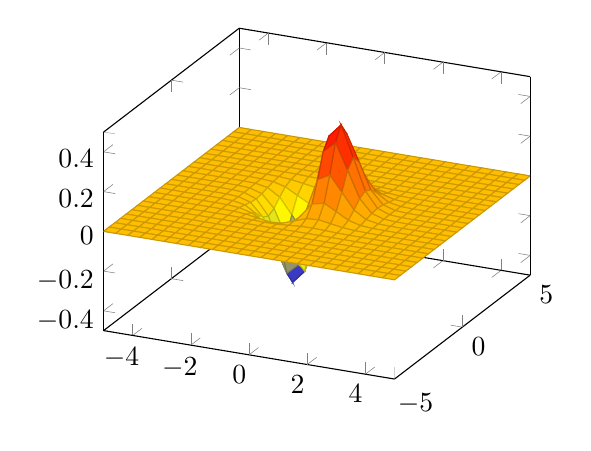
\begin{tikzpicture}
    \begin{axis}
      \addplot3[
      surf,
      ]{exp(-x^2-y^2)*x};
    \end{axis}
  \end{tikzpicture}
We now get to some more details on 2D plot.
\clearpage
\section{2D Plot}
What the heck...Let's do some damage!

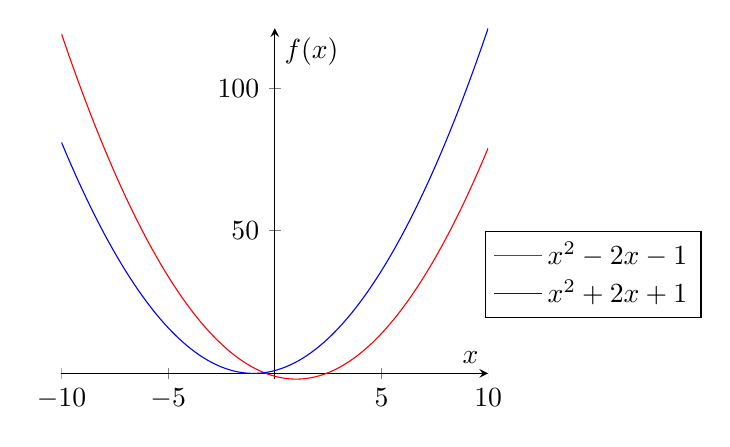
\begin{tikzpicture}
  \begin{axis}[
    axis lines= center,
    xlabel= $x$,
    ylabel= {$f(x)$},
    legend style={at={(axis cs:20,50)},anchor=north east},
    ]
    %We now add a red parabola
    \addplot[
    domain=-10:10,
    samples=100,
    color=red,
    ]
    {x^2-2*x-1};
    \addlegendentry{$x^2-2x-1$}
    %Now we add another parabola to the same axis
    \addplot[
    domain=-10:10,
    samples=100,
    color=blue
    ]
    {x^2+2*x+1};
    \addlegendentry{$x^2+2x+1$}
  \end{axis}
\end{tikzpicture}

Come on man!!!! Let's make some plots from data.
\clearpage
\subsection{Plotting from data}
I love to test \textcelsius

\begin{tikzpicture}
  \begin{axis}[
    title={Temperature dependence of CuSO$_4$\cdot5H$_2$O},
    xlabel={Temperature [\textcelsius]},
    ylabel={Solubility [g per 100g water]},
    xmin=0, xmax=100,
    ymin=0, ymax=120,
    xtick={0,20,...,100},
    ytick={0,20,...,120},
    legend pos=north west,
    ymajorgrids=true,
    grid style=dashed,
    ]

    \addplot[
      color=blue,
      mark=square,
    ]
    coordinates {
    (0,23.1)(10,27.5)(20,32)(30,37.8)(40,44.6)(60,61.8)%
    (80,83.8)(100,114)
    };
    \addlegendentry{CuSO$_4$\cdot5H$_2$0}
  \end{axis}
\end{tikzpicture}

When the data is in a file, put
\verb+\addplot table {file_with_the_data.dat}+
instead of using \verb+\addplot coordinates {}+.

\subsection{Scatter plots}
Scatter plot is used to represent information by using
some kind of marks, which are common, for example,
when computing statistical regression.

\begin{tikzpicture}
  \begin{axis}[
    enlargelimits=false,
    ]

    \addplot+[
    only marks,
    scatter,
    mark=halfcircle*,
    mark size=2.9pt,
    ]
    table[meta=ma]{data.dat};
  \end{axis}
\end{tikzpicture}

\subsection{Bar graphs}
Bar graphs are used to display gathered data.

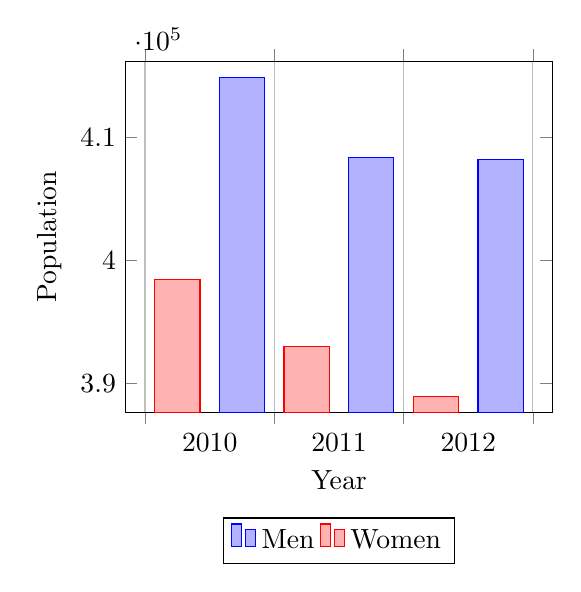
\begin{tikzpicture}
  \begin{axis}[
    x tick label style={
      /pgf/number format/1000 sep=},
    ylabel=Population,
    xlabel=Year,
    enlargelimits=0.05,
    legend style={at={(0.5,-0.3)},
    anchor=north, legend columns=2},
    ybar interval=0.7,
    ]

    \addplot
      coordinates {(2012,408184)(2011,408348)
      (2010,414870)(2009,412576)};
    \addplot
      coordinates {(2012,388950)(2011,393007)
      (2010,398449)(2009,395972)};
    \legend{Men,Women}
  \end{axis}
\end{tikzpicture}

\section{3D Plots}
For the basic plot, we refer to section~\ref{sec:1}. We now
use mesh feature for the plot.

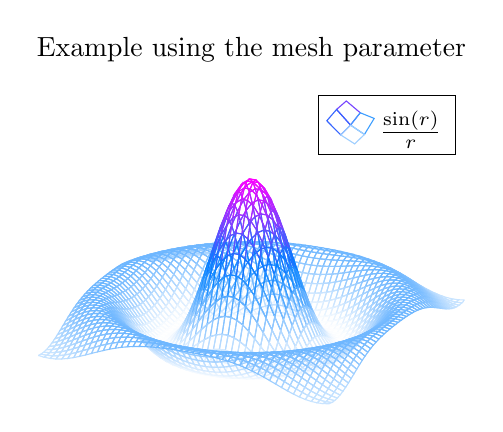
\begin{tikzpicture}
  \begin{axis}[
      title=Example using the mesh parameter,
      colormap/cool,
      hide axis,
    ]

    \addplot3[
    mesh,
    samples=50,
    domain=-8:8,
    ]
    {sin(deg(sqrt(x^2+y^2)))/sqrt(x^2+y^2)};
    \addlegendentry{$\frac{\sin(r)}{r}$}
  \end{axis}
\end{tikzpicture}

\subsection{Contour plot}
  The data needs to be calculated by external programs(%
  gnutplot, mathematica, etc\ldots)

  \begin{tikzpicture}
    \begin{axis}[
      title={Contour plot, view from top},
      view={0}{90},
      ]

      \addplot3[
        contour gnuplot={levels={0.8, 0.4, 0.2, -0.2}}
      ]
      {sin(deg(sqrt(x^2+y^2)))/sqrt(x^2+y^2)};
    \end{axis}
  \end{tikzpicture}

\subsection{Plotting a surface from data}
The source code for this graph should be self-explanatory.

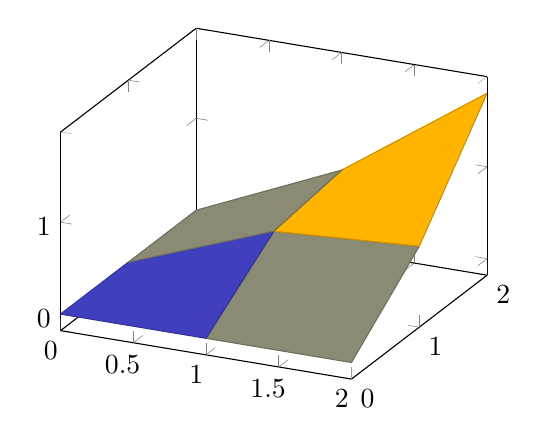
\begin{tikzpicture}
  \begin{axis}
    \addplot3[
      surf,
    ]
    coordinates {
    (0,0,0) (0,1,0) (0,2,0)

    (1,0,0) (1,1,0.6) (1,2,0.7)

    (2,0,0) (2,1,0.7) (2,2,1.8)
    };
  \end{axis}
\end{tikzpicture}

\subsection{Ploting parametric curve}
A sample of the parametric plot is here, but
I do not know what a parametric means at this moment!
Therefore, this is blindly copied from the tutorial
source.

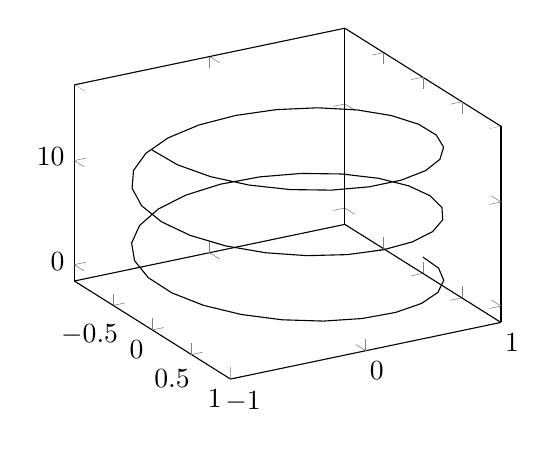
\begin{tikzpicture}
  \begin{axis}[
      view={60}{30},
    ]
    \addplot3[
      domain=0:5*pi,
      samples=60,
      samples y=0,% Preventing pgfplots from joining 2 extreme points
    ]
    ({sin(deg(x))},
     {cos(deg(x))},
     {x}%
    );
  \end{axis}
\end{tikzpicture}

\part{Tikz package}\footnote{The tutorial
is taken from \texttt{A very minimal
introduction to Tikz} by Jacques Cr\'emer}
Since Tikz and Pgfplots packages are such gigantic packages,
these intro will have to be enough until a later time.
Addtional examples will be updated later in part 3 if
I have free time, but the chances of which is virtually $0$.

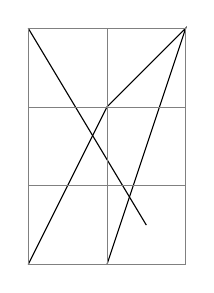
\begin{tikzpicture}
  \draw (0,0) -- (1,2) -- (2,3) -- (1,0);
  \draw (0,3) -- (1.5,0.5);
  \draw[help lines] (0,0) grid (2,3);
\end{tikzpicture}
  \hskip 5pt
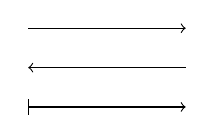
\begin{tikzpicture}
  \draw[->] (0,0) -- (2,0);
  \draw[<-] (0,-0.5) -- (2,-0.5);
  \draw[|->] (0,-1) -- (2,-1);
\end{tikzpicture}
  \hskip 5pt
\begin{tikzpicture}
  \draw[<->] (0,2) -- (0,0) -- (3,0);
\end{tikzpicture}
  \hskip 5pt
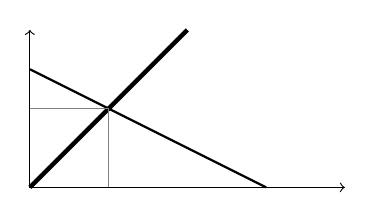
\begin{tikzpicture}
  \draw[<->] (0,2) -- (0,0) -- (4,0);
   \draw[thick] (0,1.5) -- (3,0);
  \draw[ultra thick] (0,0) -- (2,2);
  \draw[help lines] (1,0) -- (1,1) -- (0,1);
\end{tikzpicture}

Drawing is an art\ldots We can also use custom width
for draw with \verb+line width=...+The default width
unit is point(pt).


\begin{tikzpicture}
  \draw[line width=12] (0,0) -- (2,0);
  \draw[line width=0.2cm] (4,.75) -- (5,.25);
\end{tikzpicture}

Let's draw some circle.

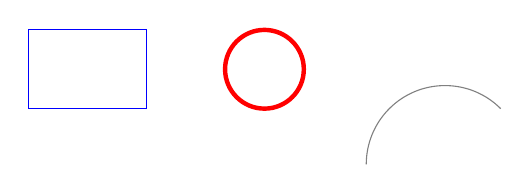
\begin{tikzpicture}
  \draw[blue] (0,0) rectangle (1.5,1);
  \draw[red,ultra thick] (3,0.5) circle [radius=0.5];
  \draw[gray] (6,0) arc [radius=1,start angle=45,
  end angle=180];
\end{tikzpicture}
\hskip 5pt
\begin{tikzpicture}
  \draw [<->, rounded corners, thick, purple]
  (0,2) -- (0,0) -- (3,0);
\end{tikzpicture}

Let's draw a curve!

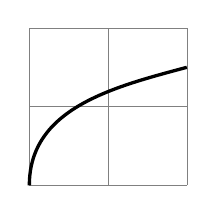
\begin{tikzpicture}
\draw[help lines] (0,0) grid (2,2);
\draw[very thick] (0,0) to [out=90,in=195] (2,1.5);
\end{tikzpicture}

Let's plot some functions!

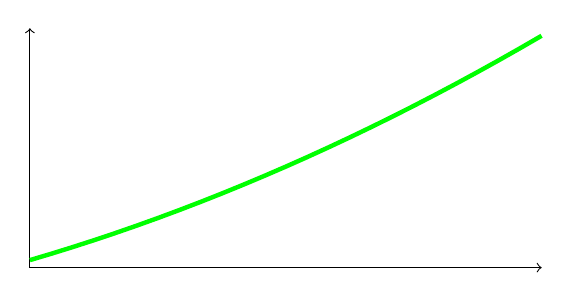
\begin{tikzpicture}[xscale=13,yscale=3.8]
  \draw[<->] (0,0.8)--(0,0)--(0.5,0);
  \draw[green,ultra thick,domain=0:0.5]
  plot(\x,{0.025+\x+\x*\x});
\end{tikzpicture}
\hskip 5pt
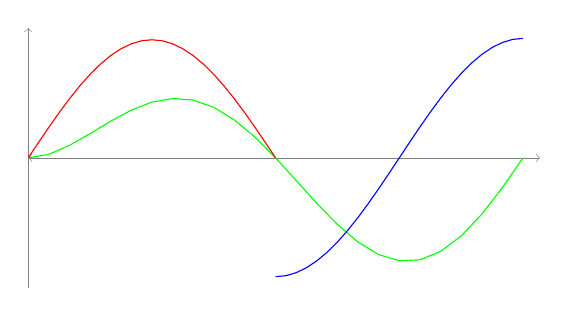
\begin{tikzpicture}[yscale=1.5]
  \draw[help lines,<->] (0,0) -- (6.5,0);
  \draw[help lines,->] (0,-1.1) -- (0,1.1);
  \draw[green,domain=0:2*pi] plot (\x,
  {(sin(\x r)*ln(\x + 1))/2});
  \draw[red,domain=0:pi] plot (\x, {sin(\x r)});
  \draw[blue,domain=pi:2*pi] plot (\x,
  {cos(\x r)*exp(\x/exp(2*pi))});
\end{tikzpicture}

Let's fill up some simple areas.

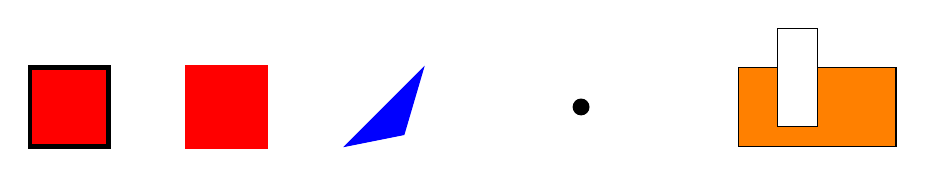
\begin{tikzpicture}
  \draw[fill=red,ultra thick] (0,0) rectangle (1,1);
  \draw[fill=red,ultra thick, red] (2,0) rectangle (3,1);
  \draw[blue, fill=blue] (4,0) -- (5,1) -- (4.75,0.15) --cycle;
  \draw[fill] (7,0.5) circle [radius=0.1];
  \draw[fill=orange] (9,0) rectangle (11,1);
  \draw[fill=white] (9.5,0.25) rectangle (10,1.5);
\end{tikzpicture}

outline or not? with \verb+\path+


\begin{tikzpicture}
  \path[fill=gray] (0,0) rectangle (1.5,1);
  \draw[fill=gray] (2,0) rectangle (3.5,1);
\end{tikzpicture}

Let's fill up some arbitrary areas:


\begin{tikzpicture}
  \draw[ultra thick] (0,0) to [out=87,in=150] (1,1)
  -- (0.85,0.15) -- cycle;
  \draw[ultra thick,fill=purple] (2,0) to [out=87,in=150]
  (3,1) -- (2.85,0.15) -- cycle;
  \path[fill=purple] (4,0) to [out=87,in=150] (5,1)
  -- (4.85,.15) --cycle;
\end{tikzpicture}

Let's put some labels in the picture.

\begin{tikzpicture}
  \draw[thick, <->] (0,2) -- (0,0) -- (2,0);
  \node at (1,1) {yes};
  \draw[thick, <->] (4,2) -- (4,0) -- (6,0);
  \node[below right] at (6,0) {$x$};
  \node[left] at (4,2) {$y$};
  \draw[fill] (4.4,.6) circle [radius=.5pt];
  \node[above right] at (4.4,.6) {$A$};
\end{tikzpicture}

Mixing the \verb+\node+ by putting it right after
the point of relative position, without the backslash
\verb+\+.

An example of alignment of text in \verb+\node+

\begin{tikzpicture}
  
\end{tikzpicture}
\end{document}
